\documentclass{article}

\usepackage[utf8]{inputenc}
\usepackage[english,russian]{babel}
\usepackage{graphicx}
\usepackage{wrapfig}

\title{1 НЕДЕЛЯ 1.47, 1.60, 1.75, 1.83}
\author{Семёнов Андрей Б02-016}

\begin{document}

\maketitle

\paragraph{1.47}
\par Путь $P=\alpha V\Rightarrow\alpha V^2=\nu RT$
\begin{displaymath}
\delta Q=\delta A+dU=PdV + C_{V}dT\Rightarrow C=\frac{\delta Q}{dT}=C_{V}+\frac{PdV}{dT}=\alpha\frac{VdV}{dT}+C_{V}
\end{displaymath}
Таким образом
\begin{displaymath}
C=\frac32\nu RT + \alpha\frac{dV^2}{dT}=\frac32\nu RT + \frac\alpha2\frac{d(\nu RT/2)}{dT}=\frac R2 +C_{V}
\end{displaymath}
\textbf{Ответ:} $C=C_{V}+\frac R2$


\paragraph{1.60}
\par Работа нагретого газа по передвижению поршня равна изменению внутренней энергии ненагретой части сосуда. Для этой части процесс является адиабатическим сжатием так, как при подведении тепла, количество теплоты не изменяется(поршень телонипроницаемый).
\begin{figure}[h]
\begin{minipage}[h]{0.49\linewidth}
\center{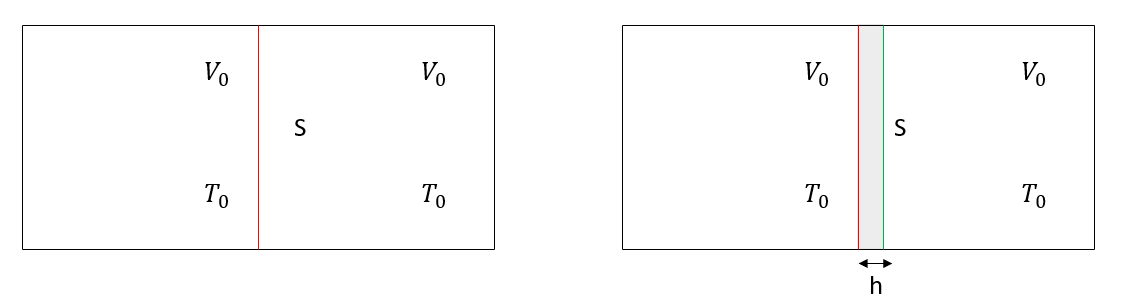
\includegraphics[width=2\linewidth]{160}}
\end{minipage}
\end{figure}
\begin{displaymath}
dU_{2}=\frac{P_{0}V_{0}}{\gamma -1}(\frac VV_{0}^{\gamma -1}-1)
\end{displaymath}
Внутрення энергия это функция состояния, поэтому для нагретого сосуда выполняется:

\begin{displaymath}
dU_{1}=\frac{C_{V}}{R}(P(V_{0}+Sh)-P_{0}V_{0})
\end{displaymath}

Вспомним, про связь $P$ и $V$ в адибатическом процессе:

\begin{displaymath}
\frac {P}{P_{0}}=(\frac{V_{0}}{V_{0}-Sh})^{\gamma}
\end{displaymath}

Таким образом, количество затраченного тепла равняется сумме этих внутренних энергий:

\begin{displaymath}
Q=dU_{1}+dU_{2}=\frac{2RT_{0}}{\gamma-1}(\frac{V_{0}}{V_{0}-Sh}-1)
\end{displaymath}
\textbf{Ответ:} $Q=\frac{2RT_{0}}{\gamma-1}(\frac{V_{0}}{V_{0}-Sh}-1)$


\paragraph{1.75}
\par $PV^\gamma=const$ и $PV\sim T$, тогда:
\begin{displaymath}
PV\cdot V^{\gamma-1}\sim TV^{\gamma-1}\sim T(\frac TP)^{\gamma-1}\sim T^\gamma P^{1-\gamma}=const
\end{displaymath}
Получили уравнение адиабатического процесса в $P, T$ координатах. Далее выразим $T_{2}$:
\begin{displaymath}
T_{1}^{\gamma}P_{1}^{1-\gamma}=T_{2}^{\gamma}P_{2}^{1-\gamma}\Rightarrow T_{2}=T_{1}\frac{P_{1}}{P_{2}}^{\frac{1-\gamma}{\gamma}}
\end{displaymath}
Осталось вычислить показатель адиабаты $\gamma$. Так, как гелий$-$одноатомный газ, а водород$-$двухатомный, то, учитывая $\nu_{He}=2\nu{H_{2}}$, не составит труда отыскать молярнуюю теплоёмкость:
\begin{displaymath}
C_{V}=\frac{\frac32R\nu_{He} + \frac52R\nu_{H_{2}}}{\nu_{He}+\nu{H_{2}}}\Rightarrow C_{V}=\frac{11}{6}R
\end{displaymath}
Из уравнение Майера следует: \begin{displaymath}C_{P}=\frac{17}{6}R\end{displaymath}Значит показатель адиабаты $\gamma=17/11$. Используя выражение для $T_{2}$ имеем:
\begin{displaymath}
T_{2}=600\cdot(\frac81)^{\frac{1-\frac{17}{11}}{\frac{17}{11}}}=600\cdot8^{\frac{-6}{17}}\approx288
\end{displaymath}
\textbf{Ответ:} $T_{2}=288$К\\
P.S. Не могу понять, как в Овчинке получился ответ 300К... 


\paragraph{1.83}
\par На каждую молекулу приходиться два атома $I_{2}$, поэтому запишем уравнение, связывающее молярную массу с количеством молекул одноатомного и двухатомного газа:
\begin{displaymath}
2c_{P}A=2\alpha\frac52R + (1-\alpha)\frac72R\Rightarrow \alpha=\frac{4c_{P}A-7R}{3R}\Rightarrow \alpha\approx0.5
\end{displaymath}
В этой задаче гораздо удобнее проводить вычисления не в СИ, а именно в тех размерностях, которые даны в условии.\\
\textbf{Ответ:} $\alpha=0.5$
\end{document}